\documentclass[tikz,border=10pt]{standalone}
\usepackage{tikz}
\usetikzlibrary{arrows.meta, positioning}

\begin{document}
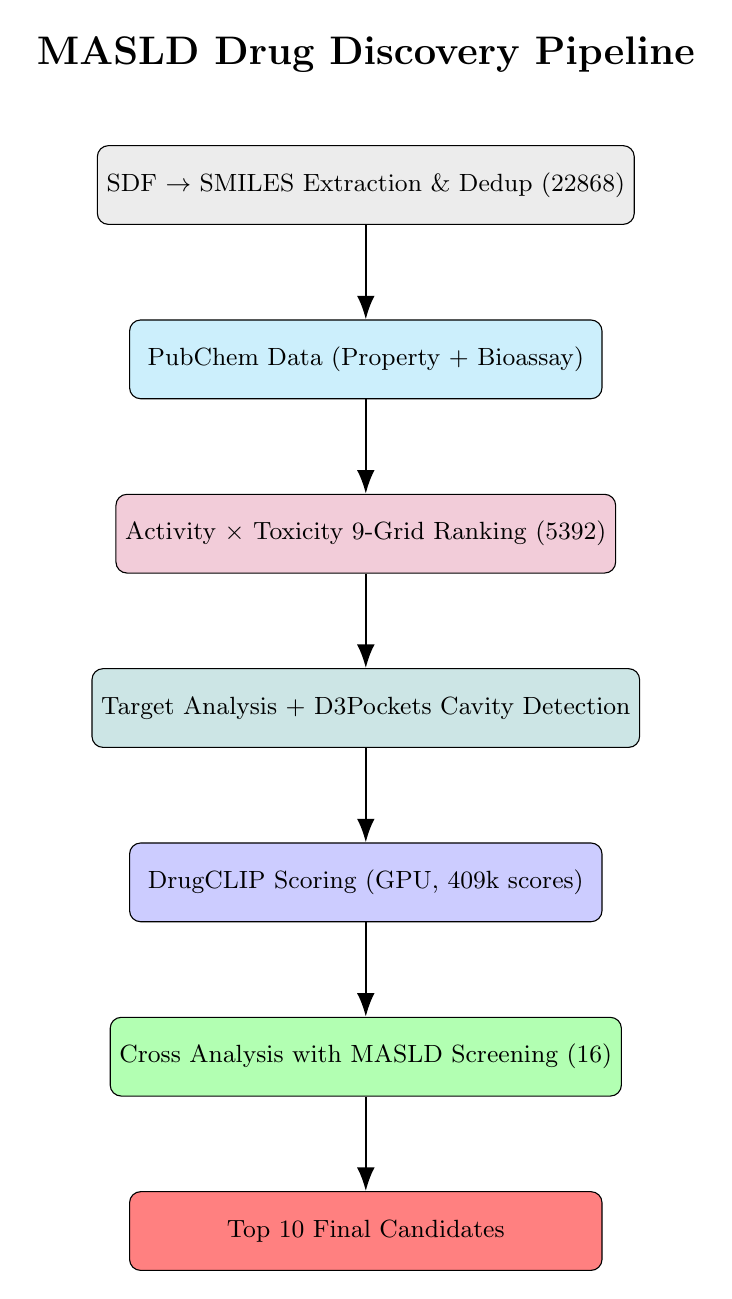
\begin{tikzpicture}[
  node distance=1.2cm,
  box/.style={rectangle, draw, rounded corners, minimum width=6cm, minimum height=1cm, align=center, font=\small, fill=#1},
  arr/.style={-{Latex[length=3mm]}, thick},
  title/.style={font=\Large\bfseries, align=center}
]

  \node[title] (title) {MASLD Drug Discovery Pipeline};

  \node[box={gray!15}, below=0.8cm of title] (p1) {SDF $\rightarrow$ SMILES Extraction \& Dedup (22868)};
  \node[box={cyan!20}, below=1.2cm of p1] (p2) {PubChem Data (Property + Bioassay)};
  \node[box={purple!20}, below=1.2cm of p2] (p3) {Activity $\times$ Toxicity 9-Grid Ranking (5392)};
  \node[box={teal!20}, below=1.2cm of p3] (p4) {Target Analysis + D3Pockets Cavity Detection};
  \node[box={blue!20}, below=1.2cm of p4] (p5) {DrugCLIP Scoring (GPU, 409k scores)};
  \node[box={green!30}, below=1.2cm of p5] (p6) {Cross Analysis with MASLD Screening (16)};
  \node[box={red!50}, below=1.2cm of p6] (p7) {Top 10 Final Candidates};

  \draw[arr] (p1) -- (p2);
  \draw[arr] (p2) -- (p3);
  \draw[arr] (p3) -- (p4);
  \draw[arr] (p4) -- (p5);
  \draw[arr] (p5) -- (p6);
  \draw[arr] (p6) -- (p7);

\end{tikzpicture}
\end{document}